\section{Methods}
\label{sec:methods}

A self-organizing recurrent neural network (SORN) was used to learn specific input patterns, given by a defined Markov chain. It was checked how well the network was able to represent the given information. \acs{sorn} uses three plasticity rules to learn the input patterns:

\begin{itemize}
\item \ACF{stdp}
\item \ACF{sn}
\item \ACF{ip}
\end{itemize}

The time in the network is discrete and there is no refractory period modeled for the neurons. In most cases $\Nsim = 20$ networks were simulated and results were averaged.

% Zitiere grand averaging paper

The source code for all the simulation experiments is based on source code from \textcite{hartmann2015s}, which is written in \texttt{Python 2.7}. The team provided a small framework for SORN simulation experiments (\href{https://github.com/chrhartm/SORN}{https://github.com/chrhartm/SORN}). A lot of code was added or rewritten, especially regarding the evaluation of the network behavior, such that it fitted to the experiments, performed in this thesis.

\subsection{Network structure}

The reservoir consists of $N^E$ excitatory and $N^I$ inhibitory neurons. Additionally, some excitatory neurons where randomly connected to a specific number of input neurons $N^U = n$, which equals the number of Markov states. The weights $w_{ij} \in [0,1]$ between the neurons were initialized randomly. The network is build with three types of connections:

\begin{itemize}
\item Excitatory-excitatory weights: $W^{EE}$, where $\sum_{j} w^{EE}_{ij} = 1$
\item Inhibitory-excitatory weights: $W^{EI}$, where $\sum_{j} w^{EI}_{ij} = 1$
\item Excitatory-inhibitory weights: $W^{IE}$, where $\sum_{j} w^{IE}_{ij} = 1$
\item Input-excitatory weights: $W^{EU}$, where $w^{EU}_{ij} = 1$ for all $i,j$
\end{itemize}

As already explained in section \ref{sec:sorn}, there are no connections modeled between inhibitory neurons. On average, $10\%$ of the possible connections in $W^{EE}$ were realized. Hence, the matrix $W^{EE}$ is sparsely connected. The matrices $W^{IE}$ and $W^{EI}$ are fully connected. Note that the weights are normalized using equation \eqref{eq:sn}, such that the incoming weights to a neuron sum up to one.

In section \ref{sec:sorn}, figure \ref{fig:sorn} shows a sketch of the structure of the reservoir network. In this thesis $n = 4$ states were used. Hence, the state space consists of $S = \{x_1, x_2, x_3, x_4\} = \{A, B, C, D\}$. Three states are no enough to test a variety of combinations, while five or more states are already to complicated for a systematic approach. Therefore, four states seemed to be a good compromise. The four states are represented with neuron populations, called clusters. In most cases the network consists of $N^E = 200$ and $N^I = 40$. Furthermore $N_{x_i}^U = 10$ input connections are used per state or input neuron.

\subsection{Modification of the intrinsic plasticity}
\label{sec:ip-mod}

While the \acs{stdp} and the \acs{sn} where applied analog to \textcite{lazar2009sorn}, the \acs{ip} rule was modified. In the original \acs{sorn} model, the target rate $H_\IP$ was fixed. \textcite{hartmann2015s} found out that the model is more robust, if the average firing rate differs slightly between neurons. Therefore, the $H_\IP$ value from equation \eqref{eq:ip} was replaced by an individual $H_i^\IP$ target rate for every neuron $i$, resulting in

\begin{equation}
\label{eq:ip-ind}
T_i(t+1) = T_i(t) + \eta_\IP \left( x_i(t) - H_i^\IP \right).
\end{equation}

To get individual values, an average value $\bar H_\IP = 2\cdot N^U/N^E$ was used. It equals the original heuristic from \textcite{lazar2009sorn}. Additionally, a stochastic term $\varepsilon_i^\IP$ was added to the target rate of every neuron. It is uniformly \acs{iid} on an interval of $a = \sigma^\IP = 0.01$ and $b = -a = -\sigma^\IP = -0.01$. Therefore, $\varepsilon_i^\IP \sim \text{Uni}[a,b] = \text{Uni}[-\sigma^\IP,+\sigma^\IP] = \text{Uni}[-0.01,0.01]$. Together,

\begin{equation}
\label{eq:hip-ind}
T_i(t+1) = T_i(t) + \eta_\IP \left( x_i(t) - \bar H^\IP + \varepsilon_i^\IP \right)
\end{equation}

\nomenclature{$\bar H^\IP$}{Average target rate of IP mechanism}
\nomenclature{$\sigma^\IP$}{Target rate range of IP mechanism}

is the rule that was applied in the used network.

\subsection{Network training and testing}
\label{sec:train}

The network was trained in 3 phases:

\begin{itemize}
\item Self-organizing phase (plastic training phase)
\item Training phase (no-plastic training phase)
\item Testing phase
\end{itemize}

\paragraph{Self-organizing phase}

In the self-organizing phase (or plastic training phase) the input neurons are active, depending on the current sample $x_i$ from the Markov chain. In this phase all three plasticity rules are active. While STDP actively adjusts the weights, SN stabilizes the activity around every neuron without loosing the relative relationships between the neurons. IP also helps to ensure the stability of the network, since it adjusts thresholds of neurons depending on their past activity. The update of the network activity follows equation \eqref{eq:update-excitatory} for the excitatory neurons and equation \eqref{eq:update-inhibitory} for the inhibitory neurons.

During self-organizing, the information from the Markov chain is stored in the network and is coded in the weights between the neurons. Biologically, the encoding in the weights corresponds to the encoding in the strength of the synapses. In most cases the self-organizing phase was applied for $T_\plastic = 50,000$ steps. As shown below in the results, e.g. in figure \ref{fig:mc1-training}, latest after $50,000$ steps no further improvement can be noticed, in most cases much sooner.

\paragraph{Training phase}

In the training phase (or no-plastic training phase) the input neurons are still active and they still depend on the current state $x_i$ of the Markov chain. In this phase only \ac{ip} is active. Therefore, the stability of the network is ensured further on. \ac{stdp} is not active and thus also \ac{sn} is not necessary. Hence, the weights stay fixed in the training phase, meaning that $W^{EE}_{ij}(t) = W^{EE}_{ij}$ in equation \eqref{eq:update-excitatory}, where the rest of the network update equals the self-organizing phase.

The main role of the training phase is to find out how the states are represented in the activity patterns of the network after the weight structure was learned. After a burn in phase, \textcite{hartmann2015s} used the last $\tilde{T}_\compare = 2500$ steps of the no-plastic training phase for classification (see section \ref{sec:state-classification}). In the results section, it is shown that this fixed value causes a small bias, which was solved when choosing $\tilde{T}_{\text{compare}}$ more flexible, which is explained below in section \ref{sec:state-classification}.

The training phase needs enough steps to cover $\Tnoplastic > \tilde{T}_\compare$. However, the training was mostly chosen as $\Tnoplastic = 50,000$ no-plastic training steps. There are four reasons for this high value:

\begin{itemize}
\item The computational effort is very low in the training phase.
\item The number of no-plastic training steps do not influence the performance of the network (see appendix \ref{sec:appendix:noplastic}).
\item After switching off the self-organizing phase (namely the \ac{stdp} and \ac{sn}), there should be a short burn-in period. \textcite{hartmann2015s} used $\Tnoplastic = 20,000$, which seemed to be enough in all cases.
\item The updated classification algorithm, mentioned above, implies a flexible size of $\tilde{T}_\compare$, depending on the Markov chain. This change caused that a longer training phase is necessary in some cases. $\Tnoplastic = 50,000$ was enough for all applications.
\end{itemize}

\paragraph{Testing phase}

In the testing phase the input neurons are not active any more, there is no input at all. It means that $\bm v(t) = 0$ for all $t \in \{\Tevo+1, ..., \Tevo+\Ttest\}$, where $\Tevo = T_\plastic + \Tnoplastic$. Also \ac{stdp} and \ac{sn} is still switched off, as it was in the training phase before. \ac{ip} is still active. Beside the stabilizing character of the \acs{ip}, especially in the testing phase, it is responsible for spontaneous activity (see section \ref{sec:ip}). In the testing phase, the spontaneous activity patterns of the network are observed over time.

Since no input is given in this phase, it is necessary to classify the spontaneous activity patterns to a Markov state. For that purpose, the representations from the no-plastic training phase are used. A detailed explanation of the classification mechanism is given below.

The number of steps while testing has to take into account a short period of burn in. After the training phase, the input is switched off and therefore the network has to find equilibrium again, using just spontaneous activity from \acl{ip}. Mathematically, the burn in time depends on the learning rate of the \acs{ip} mechanism $\eta_\IP$. This relation is evaluated in appendix \ref{sec:appendix:eta}. In most cases the burn in phase is relatively short and $\Ttest > 20,000$ is sufficient.

\subsection{Classification of states}
\label{sec:state-classification}

In the last phase, the testing phase, it will be necessary to classify a Markov state $x_i$ to the activity pattern $\bm x(t)$ in every step of time. The activity patterns from the testing phase are compared to some representative activity patterns in the end of the no-plastic training phase.

\paragraph{Selection mechanism from Hartmann}

In \textcite{hartmann2015s} a fixed amount of $\tilde{T}_\compare = 2500$ steps in the training phase was used as representative activity patterns. From those steps the number of occurrences for every state $\tilde{T}_\compare^{x_i}$ was calculated. Let

\begin{equation}
\begin{split}
\tilde{R}_\compare &= \left\{ \bm x_u(T_\plastic+T_\noplastic-\tilde{T}_\compare), ..., \bm x_u(T_\plastic+T_\noplastic) \right\}\\
&= \left\{ \bm x_u(T_\evo-\tilde{T}_\compare), ..., \bm x_u(T_\evo) \right\}
\end{split}
\end{equation}

be a set of the last $\tilde{T}_\compare$ activity patterns in the no-plastic phase, where $u \in \{x_1, ..., x_n\}$ indicates the given input for the specific step. In order to avoid confusion, it is important to remind that the vector $\bm x_u(t)$ denotes the activity pattern of the excitatory neurons at time $t$ with input $u$ and the scalar $x_i$ denotes a state of the Markov chain. The obtained activity patterns $\tilde{R}_\compare$ are filtered by Markov state, denoted by $\tilde{R}_\compare^{x_i} = \{ \tilde{R}_\compare | u = x_i \}$. The size of this set is defined as $\tilde{T}_\compare^{x_i} = |\tilde{R}_\compare^{x_i}|$, which was mentioned above.

The minimum of those occurrences $T_\compare^\mini = \min\{\tilde{T}_\compare^{x_1}, ..., \tilde{T}_\compare^{x_n}\}$ was chosen as the number of steps for every state. If the number of representative activity patterns per state would differ, those with a higher amount of steps have a higher chance to be classified, since the amount of representative patterns cover more possible cases. Altogether, $n \cdot T_\compare^\mini$ steps are available for comparison, where $n$ is the number of Markov states or input neurons. The corresponding activity pattern for a specific state is denoted by $R_\compare^{x_i}$. To clarify how it works, a short example is provided:

Assume just two possible states $A$ and $B$, thus $n=2$. Further, assume that a Markov chain exists which provides a stationary distribution with $\pi_A = 2/5$ and $\pi_B = 3/5$. A likely sampling would result in $\tilde{T}_\compare^A = 997$ (where $\tilde{T}_\compare \cdot \pi_A = 2500 \cdot 2/5 = 1000$ would be expected) and $\tilde{T}_\compare^B = 1503$ (where $\tilde{T}_\compare \cdot \pi_B = 1500$ would be expected). Finally, in testing phase are more representative activity patterns of $B$ than $A$ available to compare with. Hence, $B$ has an advantage, compared to $A$, and activity patterns in the testing state will eventually more likely be classified as $B$. To avoid this possible bias, the minimum of both values is taken and $T_\compare^\mini = \min\{\tilde{T}_\compare^A, \tilde{T}_\compare^B\} = \min\{997,1503\} = 997$ is the number of steps which are used for \emph{every} state to compare with, meaning that $T_\compare^\mini = T_\compare^A = T_\compare^B$. Figure \ref{fig:classification-old} illustrates a similar example.

\begin{figure}
    \centering
    \begin{subfigure}{\textwidth}
    	\centering
        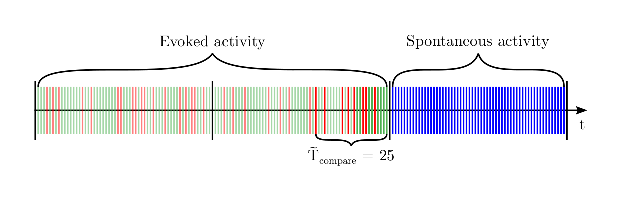
\includegraphics[width=\textwidth]{methods/classification_old}
        \vspace{5pt}
        \caption{A fixed number of potential activity patterns is chosen. In this example $\tilde{T}_\compare = 25$, meaning that the last $25$ steps in time are taken into account. In this period, state $A$ occurs $\tilde{T}_\compare^A = 8$ times and state $B$ $\tilde{T}_\compare^B = 17$ times. To ensure that the later classification of the spontaneous activity pattern have the same chance to be classified, $T_\compare^\mini = T_\compare^A = T_\compare^B = 8$ is chosen for both, state $A$ and $B$.}
        \vspace{20pt}
        \label{fig:classification-old}
    \end{subfigure}
    \begin{subfigure}{\textwidth}
    	\centering
        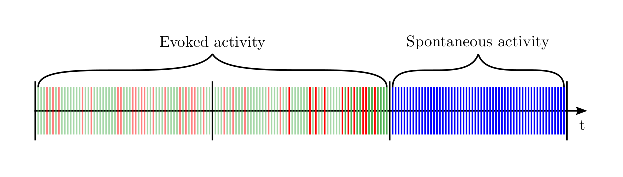
\includegraphics[width=\textwidth]{methods/classification_new}
        \vspace{5pt}
        \caption{Since the $T_\compare^\mini$ from the solution from \textcite{hartmann2015s} varies between input patterns with different probabilities, another bias needs to be taken into account when different learning patterns should be compared. Therefore, independent of the probability structure, $T_\compare = T_\compare^A = T_\compare^B = 10$ are chosen for all states. The search for those states begins at the end of the no-plastic training phase.}
        \vspace{20pt}
        \label{fig:classification-new}
    \end{subfigure}
    \caption[Selection mechanism for activity pattern representations]{Selection mechanism for activity pattern representations. In both illustrations, the first block is the plastic training phase, the second block represents the no-plastic training phase and the last block is the testing phase. Since input is given in the first two blocks, they perform with evoked activity. The last block has no input anymore and runs only with spontaneous activity from \acs{ip}. The example network is trained with two states: $A$, represented by the red lines, and $B$, drawn in green, where $\pi_A = 2/5$ and $\pi_B = 3/5$. Every line represents a point in time. The opaque lines are the selected steps, which are used as representative activity patterns for the specific state of the Markov chain. The activity of the chosen steps is collected in $R_\compare$ in general and in $R_\compare^A$ \& $R_\compare^B$ specifically. The first graphic shows the method provided by \textcite{hartmann2015s}, the second graphic illustrates the method which is applied in the network of this thesis.}
    \label{fig:classification}
\end{figure}

\paragraph{Updated selection mechanism}

While evaluating the network, another bias was found. The algorithm from \textcite{hartmann2015s} makes sure that the classification remains unbiased, if the same input pattern is chosen. But if different patterns are compared, the classification mechanism depends on the probabilities of the states. If one state in the input pattern is very rare, $T_\compare^\mini$ will be very small and therefore all activity patterns in the testing phase have just few representative patterns in the no-plastic training phase to compare with. On the other hand, if all states are equally probable, $T_\compare^\mini$ is quite high compared to the rare case. The performance between those two cases will eventually differ, just because of the number of available representative states in no-plastic training phase. In terms of Markov chains: If Markov chains with different stationary distributions are learned by the network and compared with each other, it is necessary to keep the number of $T_\compare^\mini$ constant for all chains. In section \ref{sec:input-dep-per} this effect is illustrated and discussed in detail.

An approach, which was chosen in this thesis, is to fix the number of representing steps for every state. A value of $T_\compare = 500$ was chosen. Independent of the probability of the state, starting from the end, $500$ representing activity patterns for every state were collected. If a state is very unlikely, for example with a probability of $\pi_{x_i} = 0.05$, for $500$ occurrences, $10,000$ steps are necessary in average to find enough representations for that state. Therefore, the $\Tnoplastic = 50,000$ was chosen, as indicated before. An illustration of this selection mechanism is shown in figure \ref{fig:classification-new}.

\paragraph{Classification mechanism}

After the representational activity patterns $R_\compare$ are collected with equal length $T_\compare^{x_1} = ... = T_\compare^{x_n}$, independent of the probabilities of the Markov chain, it remains to describe the classification mechanism for the activity patterns in the testing phase. First, a distance measure, the \emph{Hamming distance} is defined.

\begin{definition}[Hamming Distance]
Let $\Omega$ be an alphabet and $\bm x = (x_1, ..., x_N) \in \Omega^N$, $\bm y = (y_1, ..., y_N) \in \Omega^N$ two words with length $N \in \N$. Then the \emph{hamming distance} between those words $\bm x$ and $\bm y$ is defined as:

\begin{equation}
\label{eq:hamming}
d(\bm x, \bm y) := |\{i \in \{1, ..., N\} : x_i \neq y_i\}|
\end{equation}
\end{definition}

For the network holds that $\Omega = \{0,1\}$. The Hamming distances between every step in the testing phase $\bm x(t_\test) \in R_\test$, where $R_\test = \{ x(T_\evo + 1), ..., x(T_\evo + T_\test) \}$, and all steps in $\bm x(t_\compare) \in R_\compare$  are calculated. In that case the Hamming distance is defined as

\begin{equation}
\label{eq:hamming-applied}
d(\bm x(t_\test), \bm x(t_\compare)) = |\{ i \in \{ 1, ..., N^E \} : x_i(t_\test) \neq  x_i(t_\compare) \}|.
\end{equation}

\begin{table}[!b]
\centering
\footnotesize
\begin{tabular}{l|llllllllll|c}
$x_i$ & \multicolumn{10}{c|}{$\bm x(t_\compare)$} & $d\left(\bm x(t_\test), \bm x(t_\compare) \right)$ \\
\hline
A & \textbf{1} & \textbf{0} & 0 & \textbf{0} & \textbf{1} & 0 & \textbf{0} & 0 & \textbf{1} & 0 & 6 \\
A & 0 & \textbf{0} & 0 & \textbf{0} & 0 & \textbf{1} & \textbf{0} & \textbf{1} & 0 & \textbf{1} & 6 \\
A & 0 & 1 & 0 & \textbf{0} & 0 & \textbf{1} & \textbf{0} & \textbf{1} & \textbf{1} & 0 & 5 \\
A & 0 & \textbf{0} & \textbf{1} & \textbf{0} & 0 & \textbf{1} & 1 & 0 & \textbf{1} & \textbf{1} & 6 \\
A & 0 & \textbf{0} & 0 & 1 & 0 & 0 & \textbf{0} & \textbf{1} & \textbf{1} & \textbf{1} & 5 \\
B & 0 & 1 & \textbf{1} & \textbf{0} & 0 & 0 & 1 & 0 & 0 & 0 & 2 \\
A & 0 & 1 & 0 & 1 & 0 & \textbf{1} & \textbf{0} & \textbf{1} & \textbf{1} & \textbf{1} & 6 \\
B & 0 & 1 & \textbf{1} & 1 & 0 & 0 & \textbf{0} & 0 & 0 & 0 & 2 \\
A & \textbf{1} & \textbf{0} & 0 & \textbf{0} & 0 & \textbf{1} & 1 & \textbf{1} & \textbf{1} & \textbf{1} & 6 \\
B & \textbf{1} & 1 & \textbf{1} & 1 & 0 & 0 & 1 & 0 & 0 & \textbf{1} & 2 \\
B & 0 & \textbf{0} & \textbf{1} & 1 & 0 & 0 & \textbf{0} & 0 & 0 & 0 & 3 \\
A & \textbf{1} & 1 & 0 & \textbf{0} & 0 & 0 & 1 & \textbf{1} & \textbf{1} & \textbf{1} & 5 \\
A & 0 & \textbf{0} & 0 & \textbf{0} & 0 & \textbf{1} & \textbf{0} & \textbf{1} & \textbf{1} & \textbf{1} & 7 \\
B & 0 & 1 & \textbf{1} & 1 & 0 & 0 & 1 & 0 & 0 & 0 & \textbf{1} \\
B & 0 & 1 & \textbf{1} & \textbf{0} & 0 & 0 & \textbf{0} & \textbf{1} & \textbf{1} & 0 & 5 \\
A & 0 & \textbf{0} & 0 & \textbf{0} & 0 & 0 & \textbf{0} & 0 & 0 & \textbf{1} & 4 \\
B & 0 & \textbf{0} & \textbf{1} & 1 & 0 & 0 & \textbf{0} & 0 & 0 & 0 & 3 \\
B & \textbf{1} & 1 & \textbf{1} & 1 & 0 & 0 & \textbf{0} & \textbf{1} & 0 & 0 & 4 \\
B & 0 & 1 & \textbf{1} & 1 & 0 & 0 & \textbf{0} & \textbf{1} & 0 & 0 & 3 \\
B & 0 & \textbf{0} & 0 & 1 & 0 & 0 & 1 & 0 & 0 & 0 & \textbf{1} \\
\hline
\hline
$\bm x(t_\test)$ & 0 & 1 & 0 & 1 & 0 & 0 & 1 & 0 & 0 & 0 &  \\
\hline
$\bm u_A$ & 0 & 0 & 0 & 0 & 0 & 1 & 0 & 1 & 1 & 1 &  \\
$\bm u_B$ & 0 & 1 & 1 & 1 & 0 & 0 & 1 & 0 & 0 & 0 & 
\end{tabular}
\vspace{5pt}
\caption[State classification using Hamming distance]{State classification using Hamming distance. Shown are $T_\compare^A = T_\compare^B = 10$ representative states from the no-plastic training phase, corresponding to figure \ref{fig:classification-new}. An activity vector $\bm x(t_\test)$ and examples of input vectors $\bm u_A$ and $\bm u_B$, corresponding to the Markov states $A$ and $B$ are shown in the bottom of the table. On the right side the Hamming distance between any $\bm x(t_\compare)$ and the $\bm x(t_\test)$ is calculated. The differing digits in the vectors are bold. The smallest distance is given by two vectors corresponding to an $B$ input, with a distance of just $1$, which is highlighted in bold on the right side. Therefore, the chosen step in testing phase would be classified as $B$. This procedure is repeated for every $\bm x(t_\test) \in R_\test$.}
\label{tb:hamming}
\end{table}

The activity pattern $\bm x(t_\compare)$ with the smallest distance $d(\bm x(t_\test), \bm x(t_\compare))$ for all $t_\compare$ is chosen and denoted by $\bm x^\mini_\compare(t_\test)$. Corresponding to $\bm x^\mini_\compare(t_\test)$ exists a specific input $u \in \{x_1, ..., x_n\}$ which is chosen as the Markov state for the corresponding step $t_\test$ in the testing phase. A simple example, which gives an intuition is shown in table \ref{tb:hamming}. The process is in principle a $k$-nearest neighbors algorithm with $k=1$, where the distance between the vectors is measured using a hamming distance.

The question arises what happens if two or more patterns from training phase having equal distances, assuming that the patterns in the training phase belong to different Markov states. \textcite{hartmann2015s} solved this problem by shuffling the training states, before calculating the distances and then taking the first element which has minimum distance. With this method a systematical bias is prevented.

However, the algorithm is relatively simple, which is its strength, at least regarding computational effort and simplicity in implementation. The classification method will be examined in the results and further discussed in the discussion.

\subsection{Measuring performance}

The reservoir network is trained with a specific Markov chain, where the states in the Markov chain represent input clusters in the neural network, modeled by input neurons. Ideally, the network finds a good representation of the transition probabilities and the stationary distribution, stored in the weights, to reproduce the Markov chain. Statistically, the network can be seen as an estimator of the true probability structure of the Markov chain. An estimator in that sense can be optimized by finding better parameter configurations of the network. The approach does not include an analytic study of the estimator characteristics, rather it is a simulation study.

\nomenclature{$\hat{\bm\pi}$}{Estimated stationary distribution of a Markov chain}
\nomenclature{$\hat M$}{Estimated transition matrix of a Markov chain}

Let $M$ denote the true transition matrix and $\hat M$ the estimator of the transition matrix. Analogously, $\bm\pi$ is the true stationary distribution of the Markov chain and $\bm{\hat\pi}$ the estimator of the stationary distribution. To quantify the performance of the estimators $\hat M$ and $\bm{\hat\pi}$, a common \acf{mse} can be implemented. For a general parameter $\bm\vartheta$ and associated estimator $\hat{\bm\vartheta}$, the \ac{mse} is defined as

\begin{equation}
\label{eq:mse}
\MSE(\bm{\hat\vartheta}) = \E_{\bm{\hat\vartheta}}[(\bm{\hat\vartheta} - \bm\vartheta)^T (\bm{\hat\vartheta} - \bm\vartheta)].
\end{equation}

In both cases, $\hat M$ and $\bm{\hat\pi}$, the analytic solution is probably impossible or at least very hard to obtain, since both estimators are highly non-linear random variables. But for both estimators an estimator for the \ac{mse} can be introduced. It is based on a Monte Carlo approximation. The simulation was repeated $\Nsim$ times. For the vector parameter $\bm\vartheta \in \R^d$

\begin{equation}
\label{eq:mse-est}
\widehat{\MSE}(\bm{\hat\vartheta}) = \frac{1}{d \cdot \Nsim} \sum_{i=1}^{\Nsim} (\bm{\hat\vartheta}_i - \bm\vartheta_i)^T (\bm{\hat\vartheta}_i - \bm\vartheta_i)
\end{equation}

will be the general formulation of the used performance measure.

In case of the transition matrix $M$, a stochastic matrix, the rows need to be concatenated. Therefore, $\bm m = (p_{11}, ..., p_{1n}, p_{21}, ..., p_{2n}, p_{31}, ..., p_{nn})^T$ (compare with equation \eqref{eq:trans-matrix}) defines a vector, containing all entries from the transition matrix. Finally, the estimator of the \ac{mse} for the transition matrix estimator $\hat M$ is defined as

\begin{equation}
\varepsilon_M = \widehat{\MSE}(\bm{\hat m}) = \frac{1}{n^2 \cdot \Nsim} \sum_{i=1}^{\Nsim} (\bm{\hat m}_i - \bm m_i)^T (\bm{\hat m}_i - \bm m_i).
\end{equation}

\nomenclature{$\varepsilon_M$}{Estimated mean squared error of transition matrix}

In case of the stationary distribution, the calculation is straight forward. The estimator of the \ac{mse} for the stationary distribution estimator $\bm{\hat\pi}$ is defined as

\begin{equation}
\varepsilon_\pi = \widehat{\MSE}(\bm{\hat\pi}) = \frac{1}{n \cdot \Nsim} \sum_{i=1}^{\Nsim} (\bm{\hat\pi}_i - \bm\pi_i)^T (\bm{\hat\pi}_i - \bm\pi_i).
\end{equation}

\nomenclature{$\varepsilon_\pi$}{Estimated mean squared error of stationary distribution}

It remains to show how $\hat M$ and $\bm{\hat\pi}$ are obtained. Since an analytic representation is highly complex, the estimators are empirically obtained from the output of the network. Assuming that the states of the Markov chain in the testing phase are already classified (using the method from section \ref{sec:state-classification}), the stationary distribution can directly be calculated by taking the frequencies of the states. If $n_{x_i}$ is the number of occurrences for state $x_i$ in the testing phase, the estimator is defined by

\begin{equation}
\bm{\hat\pi} = \left( \frac{n_{x_1}}{N_\test}, ..., \frac{n_{x_n}}{N_\test} \right)^T,
\end{equation}

where $N_\test = |\{ \bm x(t_\test) \,:\, \bm x(t_\test) \neq 0 \}|$ for all $t_\test \in \{ T_\evo + 1, ..., \Tevo+\Ttest \}$ is the number of non-silent steps in the training phase, where $\bm x(t_\test)$ is an activity vector of the network, as used before. Note that $\bm x(t_\test) \neq 0$ is equivalent to $x_i(t_\test) \neq 0$ for all $i \in \{1,...,N^E\}$. Equivalently $N_\test = n_{x_1} + ... + n_{x_n} = \sum_{j=1}^n x_{x_j}$ is just the sum of all non-zero state occurrences.

To track changes in the course of the testing phase, the testing phase is split into chunks of $\Delta T_\chunk = 5000$ steps. Hence, $\bm{\hat\pi}$ is calculated for every chunk. The number of chunks $K_{\text{chunks}} = T_\test/\Delta T_\chunk$ is simply the number of overall steps in the testing phase divided by the chunk size. Again, $N_\test^k = |\{ \bm x(t_\test^k) \:|\, \bm x(t_\test^k) \neq 0 \}|$ for all $k \in \{ 1, ..., K_{\text{chunks}} \}$ describes the number of non-silent steps in every chunk $k$. The calculation of the estimator $\bm{\hat\pi}^k$ for a specific chunk $k$, changes to

\begin{equation}
\bm{\hat\pi}^k = \left( \frac{n_{x_1}^k}{N_\test^k}, ..., \frac{n_{x_n}^k}{N_\test^k} \right)^T.
\end{equation}

For the calculation of the estimator for the transition matrix, the silent steps are ignored, too. If $n_{x_i, x_j}^k$ denotes the number of transitions from state $x_i$ to state $x_j$ inside of chunk $k$, $\hat M^k$ is calculated as

\begin{equation}
\label{eq:transition-estimation}
\hat M^k = \left(\frac{n_{x_i, x_j}^k}{N_\test^k}\right)_{x_i,x_j \in S} = \begin{bmatrix}
\frac{n_{x_1,x_1}^k}{N_\test^k} & \frac{n_{x_1,x_2}^k}{N_\test^k} & \hdots  & \frac{n_{x_1,x_n}^k}{N_\test^k}\\
\frac{n_{x_2,x_1}^k}{N_\test^k} & \ddots &  & \vdots \\
\vdots &  & \ddots & \vdots \\
\frac{n_{x_n,x_1}^k}{N_\test^k} & \hdots & \hdots & \frac{n_{x_n,x_n}^k}{N_\test^k}
\end{bmatrix}.
\end{equation}

Finally, the \ac{mse} estimator can be applied. As the estimator of the stationary distribution $\bm{\hat\pi}$ just contains information about how often a state occurs, the estimated transition matrix also contains information about the transition properties. Therefore, the $\widehat{\MSE}(\bm{\hat m})$ is preferred in the following.

As a remark, it should be stated that also the hamming distance can be used as a performance measure. If the mean of the hamming distance of all steps in testing phase is calculated, it should be smaller for networks which perform better, since the learned states should be closer to the initial states. Since the differences in the hamming distance means do not differ much between different settings (see appendix \ref{sec:appendix:hamming}), this kind of performance measure was not further investigated.

A last problem was the amount of silent passes. The more silent passes exist, the worse will be the estimator. This problem was solved by just implementing a threshold. If the number of silent steps exceeded a threshold of $25\%$ of $\Delta T_\chunk$, which means that if $1 - N_\test^k/\Delta T_\chunk > 0.25$ for any $k$, an error is thrown and the network simulation is canceled.

